\documentclass[10pt]{beamer}

%%%
% PREAMBLE FOR THIS DOC 
%%%
%https://tex.stackexchange.com/questions/68821/is-it-possible-to-create-a-latex-preamble-header
\usepackage{/Users/miw267/Repos/csci246_spring2025/slides/preambles/beamer_preamble_for_CSCI246}


%%% TRY TO RESHOW TOC AT EACH SECTION START (with current section highlighted)
% Reference: https://tex.stackexchange.com/questions/280436/how-to-highlight-a-specific-section-in-beamer-toc
\newcommand\tocforsect[2]{%
  \begingroup
  \edef\safesection{\thesection}
  \setcounter{section}{#1}
  \tableofcontents[#2,currentsection]
  \setcounter{section}{\safesection}
  \endgroup
}


%%%% HERES HOW TO DO IT CORRECTLY
% FIRST IN .STY FILE, DO
%\usetheme[sectionpage=none]{metropolis}
% THEN AT EACH SECTION DO
%\begin{frame}{Outline}
%  \tableofcontents[currentsection]	
%\end{frame}



%\setbeamertemplate{navigation symbols}{}
%\setbeamertemplate{footline}[frame number]{}


%%%
% DOCUMENT
%%%

\begin{document}

%\maketitle

%% Title page frame
%\begin{frame}
%    \titlepage 
%\end{frame}



\title{04/09/2025: Graph Theory Fundamentals}
\author{CSCI 246: Discrete Structures}
\date{Textbook reference: Sec 47, Scheinerman}

\begin{frame}
    \titlepage 
\end{frame}


\begin{frame}
\small
\begin{mygreenbox}[title=Graded Quiz Pickup]
Quizzes are in the front of the room, grouped into four bins (A-G, H-L, M-R, S-Z) by last name. The quizzes are upside down with your last name on the back. Come find yours before, during, or after class. Only turn the quiz over if it's yours.
\end{mygreenbox} 
\vfill 
%\begin{myredbox}[title=Friday's Problems Quiz]
%The problems quiz on Friday (04/02) will cover:
%\begin{itemize}
%\item Conditional Probability and Independence
%\item Random Variables
%\item Expectations	
%\end{itemize}
%
%\end{myredbox}
\vfill 
\begin{myyellowbox}[title=Today's Agenda]
\begin{itemize}
	\item Reading quiz (5 mins)
	\item Review problems quizzes (15 mins)
	\item Mini-lecture ($\approx$ 10 mins)
	\item Group exercises ($\approx$ 15 mins)
\end{itemize}


\end{myyellowbox}
\vfill 

\end{frame}






\begin{frame}[standout]
Feedback on Monday's Quiz
\end{frame}


\begin{frame}{Reading Quiz Scores}
\small 
\begin{figure}[ht]
        \centering
        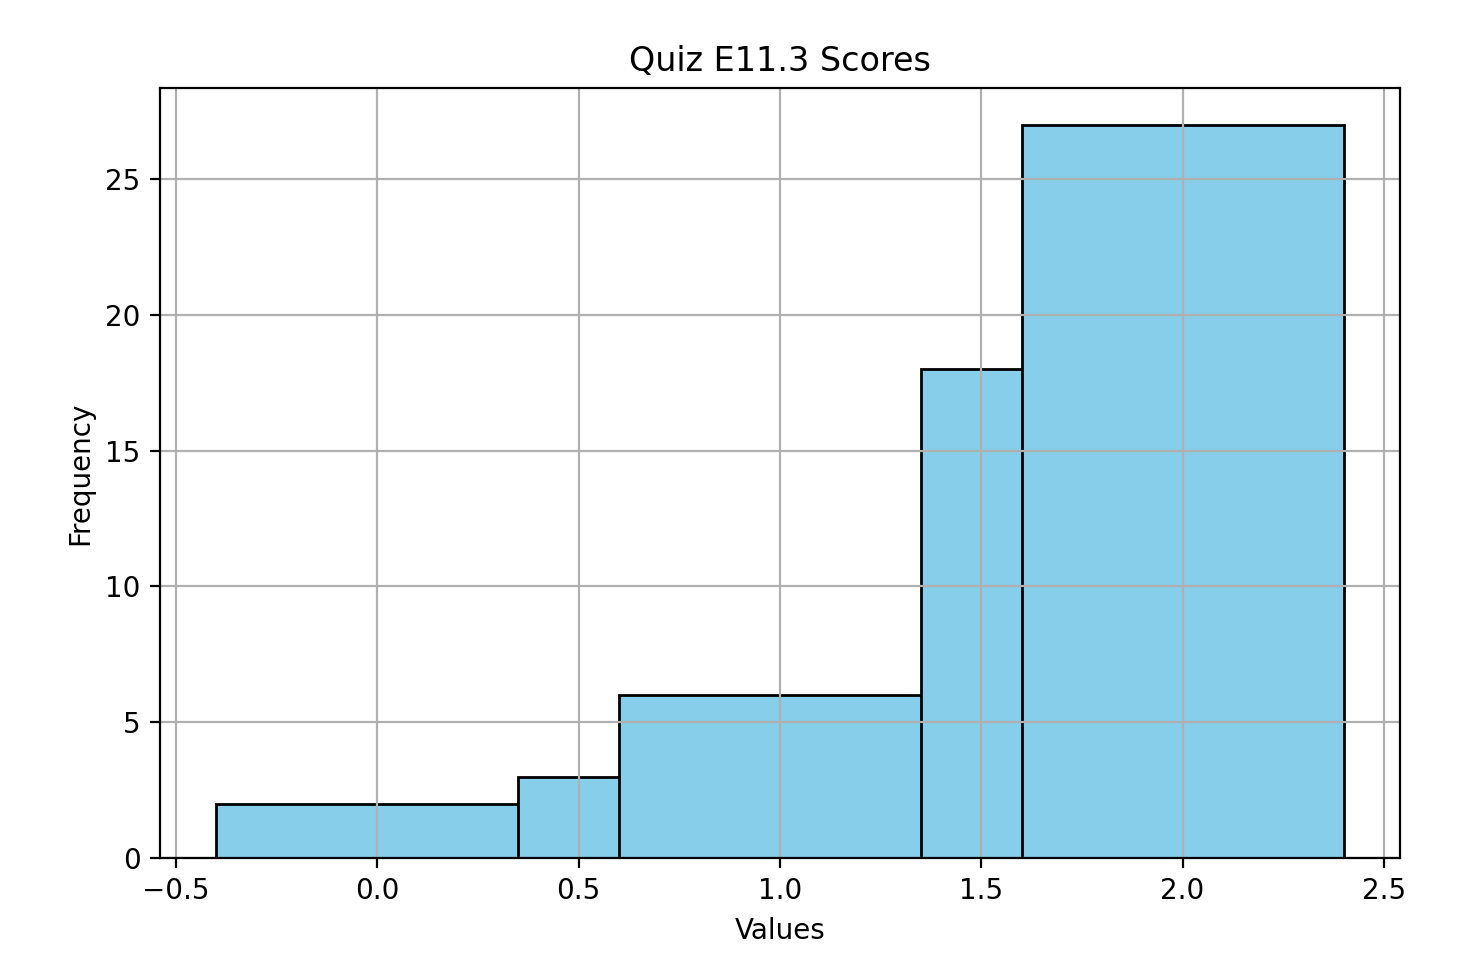
\includegraphics[width=.6\textwidth]{images/reading_quiz_scores}
   		 \caption{Median Score = 1.75/2 (87.5\%)}
\end{figure}
\vfill 
\textbf{Grading Rubric:}  
\begin{enumerate}
\item (1 point) Needed to give  reasonable answer to number of elementary operations (for the WHOLE algorithm snippet).
\item (1 point) Stating the order (ideally as Big Theta, but Big O was accepted)
\end{enumerate}


\end{frame}	




\begin{frame}[standout]
Today's reading quiz
\end{frame}

\begin{frame}
\small 
\begin{myredbox}[title=Reading Quiz (Graph Theory Fundamentals)]

\begin{enumerate}
\item What is the degree of vertex 1 in the graph below?	
\begin{figure}
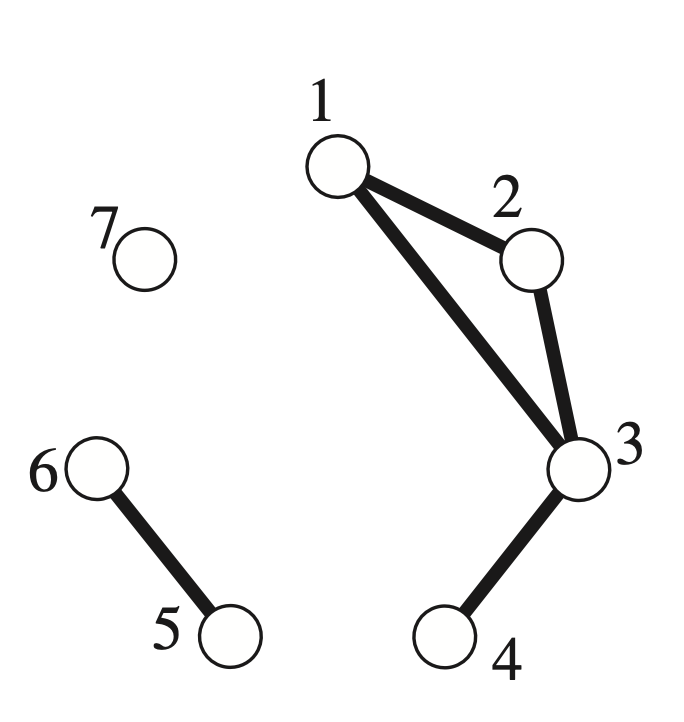
\includegraphics[width=.4\textwidth]{images/simple_graph.png}	
\end{figure}
\item Let $G=(V,E)$.  The sum of the degree of vertices in G is \textit{how many} times the number of edges? That is, if we write
\[ \sum_{v \in V} d(v) = C|E|, \]
what is $C$?
\item Give a brief explanation for your answer to number 2.
\end{enumerate}


\end{myredbox}
\end{frame}


\begin{frame}[standout]
Review for Friday's Problems Quiz
\end{frame}



\begin{frame}[standout]
Thoughts On Graph Theory Fundamentals
\end{frame}


\begin{frame}{Graphs as abstractions: The Bridge of K\text{\"o}nigsberg.}

\small 

\begin{minipage}{.47\textwidth}

\onslide+<1->\begin{figure}
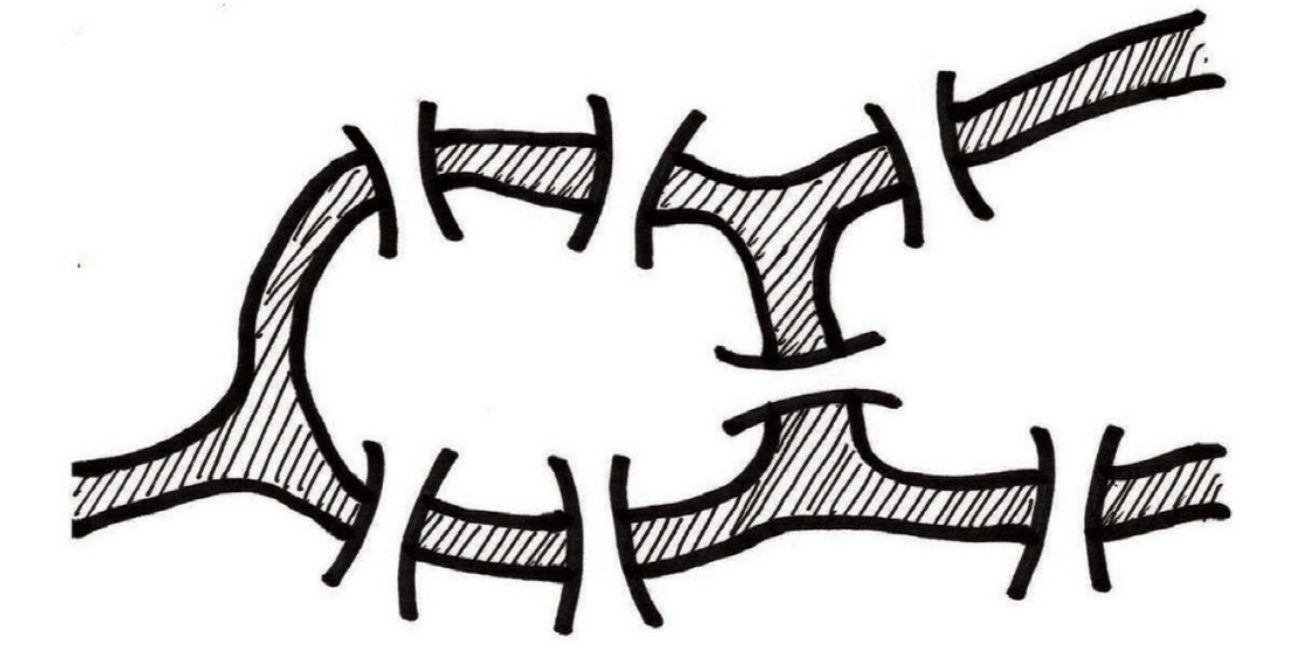
\includegraphics[width=.8\linewidth]{images/konigsberg.png}	
\caption{Bridge of K\text{\"o}nigsberg.}
\end{figure}
\end{minipage} %
\hfill 
\begin{minipage}{.47\textwidth}
\onslide+<3->\begin{figure}
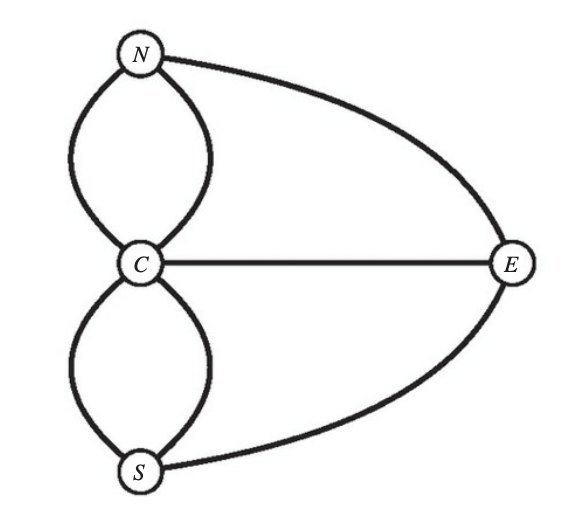
\includegraphics[width=.8\linewidth]{images/konigsberg_graph.png}
\caption{Graph representation}	
\end{figure}

\end{minipage} %

\vfill 
\onslide+<1-> \colorbox{green!30}{\textbf{Claim.}}  There was a pub on the center
island, with challenges and late-night attempts to “walk the bridges,” to make a tour of the town crossing every bridge exactly once. Despite the accompanying boasts, rarely reproducible in the sober morning, this was a difficult task.  Most who attempted found that they had missed a bridge or that they crossed a bridge twice.
\vfill 
\onslide+<2-> \colorbox{red!30}{\textbf{Question.}} Can you find a tour of the town that traverses each of the seven bridges exactly once? \hfill \onslide+<4-> \href{https://www.youtube.com/watch?v=C7YrMRdLkqo}{\underline{\blue{Click here for short video.}}}
\end{frame}

\begin{frame}[standout]
Group exercises
\end{frame}

\begin{frame}
\footnotesize 
\vfill 
\begin{columns}
\begin{column}{0.33\textwidth}
aaron.loomis: 14 \\ 
adam.wyszynski: 9 \\ 
alexander.goetz: 11 \\ 
alexander.knutson: 7 \\ 
anthony.mann: 1 \\ 
blake.leone: 20 \\ 
bridger.voss: 20 \\ 
caitlin.hermanson: 3 \\ 
cameron.wittrock: 6 \\ 
carsten.brooks: 2 \\ 
carver.wambold: 17 \\ 
colter.huber: 2 \\ 
conner.reed1: 15 \\ 
connor.mizner: 17 \\ 
connor.yetter: 4 \\ 
derek.price4: 18 \\ 
devon.maurer: 19 \\ 
emmeri.grooms: 7 \\ 
erik.moore3: 8 \\ 
ethan.johnson18: 13 \\ 
evan.barth: 10 \\\end{column}
\begin{column}{0.33\textwidth}
evan.schoening: 15 \\ 
griffin.short: 14 \\ 
jack.fry: 10 \\ 
jacob.ketola: 12 \\ 
jacob.shepherd1: 16 \\ 
jada.zorn: 13 \\ 
jakob.kominsky: 11 \\ 
james.brubaker: 14 \\ 
jeremiah.mackey: 19 \\ 
jett.girard: 3 \\ 
john.fotheringham: 3 \\ 
jonas.zeiler: 21 \\ 
joseph.mergenthaler: 10 \\ 
joseph.triem: 8 \\ 
julia.larsen: 8 \\ 
justice.mosso: 6 \\ 
kaden.price: 5 \\ 
lucas.jones6: 9 \\ 
luka.derry: 12 \\ 
luke.donaldson1: 4 \\\end{column}
\begin{column}{0.33\textwidth}
lynsey.read: 13 \\ 
mason.barnocky: 11 \\ 
matthew.nagel: 6 \\ 
micaylyn.parker: 1 \\ 
michael.oswald: 21 \\ 
nolan.scott1: 5 \\ 
owen.obrien: 7 \\ 
pendleton.johnston: 1 \\ 
peter.buckley1: 9 \\ 
reid.pickert: 19 \\ 
ryan.barrett2: 18 \\ 
samuel.hemmen: 2 \\ 
samuel.mosier: 16 \\ 
samuel.rollins: 5 \\ 
sarah.periolat: 4 \\ 
timothy.true: 12 \\ 
tristan.nogacki: 20 \\ 
tyler.broesel: 18 \\ 
william.elder1: 16 \\ 
yebin.wallace: 17 \\ 
zeke.baumann: 15 \\\end{column}
\end{columns}
\vfill
\end{frame}

\begin{frame}{Group exercises}
\small 
\noindent
\begin{minipage}[c]{0.6\textwidth}
\begin{enumerate}
	\item  Write the graph in the top figure as a pair of sets $(V, E)$.
	\item Draw a picture of the graph below
	  \resizebox{\linewidth}{!}{$
	   \bigg( \set{a,b,c,d,e}, \; \bigg\{  \set{a,b}, \set{a,c}, \set{a,d}, \set{b,e}, \set{c,d} \bigg\} \bigg) 	
	$.}
    \item Construct a graph for which the is-adjacent relation, $\sim$, is transitive.
    \item How many edges are in $K_n$, a complete graph with $n$ vertices?
    \item How many different graphs can be formed with vertex set $V=\set{1,2,3,\hdots,n}$?
    \item Prove that in every graph, the number of vertices with odd degree is even. (For example, the graph from the reading quiz, reproduced in the bottom figure, has exactly four vertices of odd degree.)
\end{enumerate}
\end{minipage}%
\hfill
\begin{minipage}[c]{0.38\textwidth}
    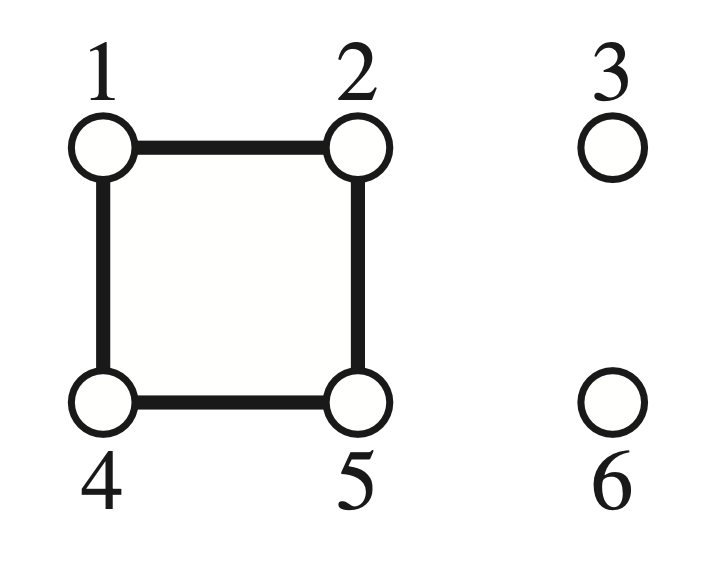
\includegraphics[width=\textwidth]{images/simple_graph_2} %
    \vfill 
    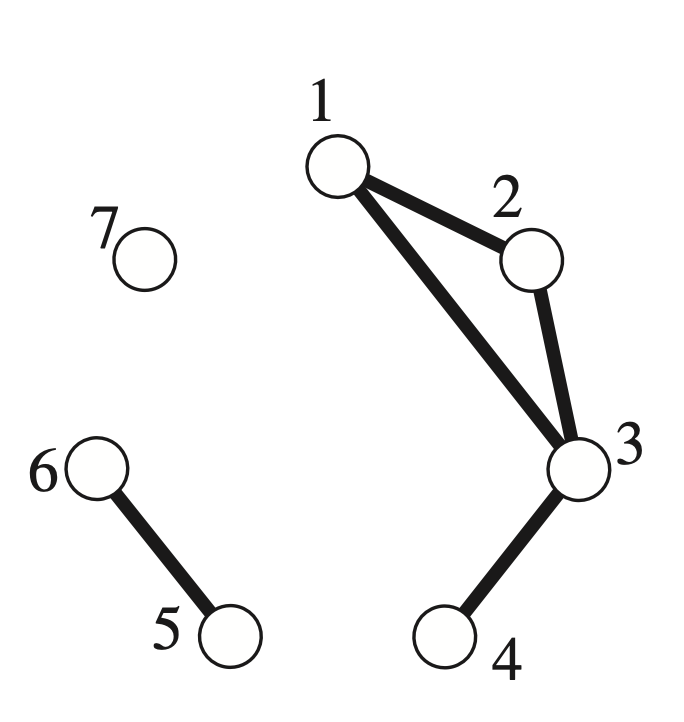
\includegraphics[width=\textwidth]{images/simple_graph.png}
\end{minipage}%    

\end{frame}




\end{document}
